\documentclass[lettersize,journal]{IEEEtran}
\usepackage{amsmath,amsfonts}
\usepackage{algorithmic}
\usepackage{algorithm}
\usepackage{array}
\usepackage[caption=false,font=normalsize,labelfont=sf,textfont=sf]{subfig}
\usepackage{textcomp}
\usepackage{stfloats}
\usepackage{url}
\usepackage{verbatim}
\usepackage{graphicx}
\usepackage{cite}
\usepackage{xspace}

\newcommand{\etal}{\textit{et al.\xspace}}

\begin{document}

\title{VERA: Generating Visual Explanations of Two-Dimensional Embeddings via Region Annotation}

\author{Pavlin G. Poli\v{c}ar, Bla\v{z} Zupan
% <-this % stops a space
\thanks{P. G. Poli\v{c}ar is with the Faculty of Computer and Information Science, University of Ljubljana.}% <-this % stops a space
\thanks{B. Zupan is with the Faculty of Computer and Information Science, University of Ljubljana and the Baylor College of Medicine.}}

% The paper headers
\markboth{}%
{Poli\v{c}ar and Zupan: VERA: Generating Visual Explanations of Two-Dimensional Embeddings via Region Annotation}

\IEEEpubid{}
% Remember, if you use this you must call \IEEEpubidadjcol in the second
% column for its text to clear the IEEEpubid mark.

\maketitle

\begin{abstract}
Two-dimensional embeddings obtained from dimensionality reduction techniques, such as MDS, t-SNE, and UMAP, are widely used across various disciplines to visualize high-dimensional data. These visualizations provide a valuable tool for exploratory data analysis, allowing researchers to visually identify clusters, outliers, and other interesting patterns in the data. However, interpreting the resulting visualizations can be challenging, as it often requires additional manual inspection to understand the differences between data points in different regions of the embedding space. To address this issue, we propose Visual Explanations via Region Annotation (VERA), an automatic embedding-annotation approach that generates visual explanations for any two-dimensional embedding. VERA produces informative explanations that characterize distinct regions in the embedding space, allowing users to gain an overview of the embedding landscape at a glance. Unlike most existing approaches, which typically require some degree of manual user intervention, VERA produces static explanations, automatically identifying and selecting the most informative visual explanations to show to the user. We illustrate the usage of VERA on a real-world data set and validate the utility of our approach with a comparative user study. Our results demonstrate that the explanations generated by VERA are as useful as fully-fledged interactive tools on typical exploratory data analysis tasks but require significantly less time and effort from the user.
\end{abstract}

\begin{IEEEkeywords}
Dimensionality reduction, Embedding, Visualization, Visual explanation, Explainable AI
\end{IEEEkeywords}

\section{Introduction}
% Why is dimensionality reduction important?
\IEEEPARstart{T}{wo-dimensional}, point-based visualizations of high-dimensional data are ubiquitous throughout various domains of science, including biology, economics, chemistry, political science, astronomy, and physics~\cite{Liu2017}.
With the advent of big data, analyzing data sets with tens of thousands of features and millions of samples has now become a commonplace occurrence.
A common step during exploratory data analysis is the visualization of these high-dimensional data sets. 
Today, data science practitioners have at their disposal a plethora of scalable dimensionality reduction methods that can be used to reduce data to two dimensions, including principal components analysis (PCA)~\cite{Jolliffe2002}, linear discriminant analysis (LDA)~\cite{Fisher1936}, FreeViz~\cite{Demsar2007}, multidimensional scaling (MDS)~\cite{Kruskal1978}, t-distributed stochastic neighbor embedding (t-SNE)~\cite{Maaten2008}, and uniform manifold approximation and projection (UMAP)~\cite{McInnes2018}.
These are routinely used to visually uncover underlying structure, such as clusters, transitions, or outliers, and to support exploratory data analysis and hypothesis generation.

% Why is the interpretation of visualizations hard?
After performing dimensionality reduction, analysts typically examine the resulting visualization to identify any discernible visual patterns and interpret how these reflect underlying phenomena in the data.
Linear methods, such as PCA, LDA, and FreeViz, offer intuitive interpretations since their inferred dimensions correspond to linear combinations of the original features. However, these are often too limited in the types of high-dimensional structures they can reveal.
Nonlinear methods, such as MDS, t-SNE, and UMAP, can reveal more complex patterns and relationships, but relating the obtained embedding dimensions to the original features becomes more challenging.
Moreover, with the development of increasingly scalable dimensionality reduction techniques~\cite{McInnes2018,Linderman2019,Lambert2022}, analysts often generate multiple embeddings using different parameter settings and algorithms, each potentially revealing different aspects of the underlying data manifold~\cite{Kobak2019}.
Each resulting embedding must then be inspected and interpreted, a task that is both time consuming and repetitive.

% What are existing approaches, and why aren't they good enough?
Existing research on interpreting two-dimensional embeddings has mostly focused on developing comprehensive interactive tools that help analysts explore every facet of resulting embeddings~\cite{}.
While these tools enable a detailed exploration of each particular embedding, the primary goal of EDA is often to obtain a high-level overview of the recovered structure rather than detailed investigation of each visual pattern.
Although many tools offer features to speed-up and assist in the exploration process, e.g. automatic clustering or feature ranking, analysts must still actively navigate and make sense of the embedding, which is both cumbersome and time-consuming.
A typical workflow might involve selecting a group of data points, inspecting their feature distributions, comparing these to the remaining data points, and annotating the visualization accordingly. This must, of course, be repeated for each interesting group of data points in each resulting embedding.
Given the repetitive nature of this task, well-designed static approaches that require no user interaction can both speed up the interpretation process and reduce cognitive load on analysts.
%While the analyst still needs to examine the outputs, doing so requires significantly less time and effort.
%Static tools can also be easily integrated into automated pipelines, generating embedding explanations as a by-product. 
%Once a particularly informative embedding is identified, the analyst can then turn to a more comprehensive interactive tool for deeper exploration of the embedding space.

% How do we solve the problem?
In this work, we propose \textit{Visual Explanations via Region Annotation (VERA)}, an automated embedding annotation tool for generating static visual explanations of two-dimensional embeddings.
VERA automatically identifies and highlights features associated with distinct regions of the embedding, presenting them in a concise, small-multiple fashion. This approach helps analysts quickly and easily obtain a high-level overview of the obtained embedding.
While a handful of static explanation approaches have already been proposed, these are often limited to a single explanation~\cite{DaSilva2015,VanDriel2020,Tian2021} or require the user to sift through a large number of output visualizations~\cite{Faust2019,Plumb2020}.
A single explanation is often insufficient for explaining all relevant visual structures while requiring users to inspect a large number of visualizations diminishes much of their efficiency over interactive tools.
In contrast, VERA generates a small set of highly informative visualizations, retaining the speed and simplicity of static visualizations without sacrificing the informativeness of interactive approaches in common exploratory data analysis tasks.
To validate our approach, we conducted a user study comparing VERA to interactive tools for embedding interpretation, and found that users given explanations generated by VERA performed as well as users with access to comprehensive, interactive tools on several common, high-level embedding interpretation tasks, while requiring significantly less time.

\section{Related Work}
\label{sec:related_work}

Alongside the development of novel dimensionality reduction approaches for the visualization of high-dimensional data~\cite{Kruskal1978,Maaten2008,McInnes2018}, numerous tools have been developed to aid in assessing the quality of the obtained embeddings~\cite{Martins2014,Stahnke2016,NonatoAupetit2019}, interpreting the resulting visual structures~\cite{ChengMueller2016,Marcilio2021,Fujiwara2020}, and comparing multiple embeddings~\cite{Arendt2020,Sivaraman2022,Boggust2022}.

Most embedding interpretation approaches aim to relate the obtained embedding to the original, high-dimensional features.
General-purpose techniques implicitly assume that the original features are, to some degree, semantically meaningful and human-interpretable.
In domains where this is not the case -- such as raw image pixels, word counts, or deep latent representations -- domain-specific solutions are often required, as in the case for text~\cite{Heimerl2016,WangHohmanChau2023} and images~\cite{Liu2019,Ye2024}.

General-purpose interpretation techniques can be broadly divided into global and local approaches.
Global approaches typically aim to express the embedding axes as linear combinations of the original features~\cite{Broeksema2013,Coimbra2016}.
While effective for linear projections, most modern dimensionality reduction techniques rely on highly non-linear transformations of the original feature space, making global approaches unsuitable for interpreting these embeddings.
Local approaches instead aim to explain local visual patterns such as clusters, transitions, and outliers and relate them to particular combinations of high-dimensional feature values.
These methods typically enrich the resulting two-dimensional scatter plot with additional graphical elements or overlays~\cite{Joia2015,ChengMueller2016,Tian2021} or provide an interactive interface through which users can navigate and explore the embedding space~\cite{Kandogan2012,Stahnke2016,Bibal2021}. Broadly speaking, local approaches can be categorized into two types: descriptive approaches and contrastive approaches.

Descriptive approaches identify regions of the embedding space, most commonly clusters, and determine which combinations of high-dimensional feature values are characteristic of the samples contained within each region.
Researchers have proposed several strategies to identify such feature combinations.
For instance, Joia \etal~\cite{Joia2015} identify salient features by examining the SVD loadings associated with each visual cluster, while Da Silva \etal~\cite{DaSilva2015} and subsequent extensions by Van Driel \etal~\cite{VanDriel2020} and Tian \etal~\cite{Tian2021} adopt a variance-based approach, identifying features that exhibit locally low variance within different embedding regions.
A similar interactive, variance-based approach was proposed by Pagliosa \etal~\cite{Pagliosa2016}.
Alternatively, some methods embed both samples and features into a shared embedding space, enabling the identification of characteristic features based on their proximity to samples in the embedding space.
For instance, Broeksema \etal~\cite{Broeksema2013} use Multiple Correspondence Analysis (MCA) to jointly embed samples and features, then identify characteristic regions using Voronoi tessellations. 
Cheng and Mueller~\cite{ChengMueller2016} developed a conceptually similar approach using MDS for joint embedding and kernel density estimation for region definition.

While descriptive approaches help explain \textit{what} particular regions correspond to, contrastive approaches aim to explain how a given region \textit{differs} from other regions. In a recent survey of sociological literature, Miller~\cite{Miller2019} highlights that humans prefer contrastive explanations and concludes that explanations in artificial intelligence should account for this preference.
Contrastive approaches generally aim to identify combinations of feature values that distinguish one region from another, and a variety of techniques have been proposed to this end.
Several approaches combine well-established statistical tools -- such as feature distribution plots~\cite{Stahnke2016,Eckelt2022}, statistical tests~\cite{Marcilio2021}, decision trees~\cite{Bibal2021}, and Shapley values~\cite{MarcilioEler2021} -- with intuitive, interactive user interfaces.
Others propose custom solutions; for example, Fujiwara \etal~\cite{Fujiwara2020} propose a contrastive variant of PCA, while Kandogan~\cite{Kandogan2012} combines several hand-crafted metrics.

Despite the plethora of existing approaches, current solutions share several notable limitations. The vast majority of these are designed as interactive tools, requiring a high degree of active user interaction which can be both repetitive and time-consuming, particularly during exploratory data analysis when the goal is to obtain a high-level overview of the embedding. This problem is especially exacerbated when inspecting and comparing multiple embeddings.
Other approaches are limited to producing a single explanation, often focusing on the single most salient combination of feature values while neglecting others, potentially interesting but less potent combinations.
Other approaches are tightly coupled to specific dimensionality reduction techniques, reducing their general applicability across methods~\cite{Chatzimparmpas2020,Broeksema2013,ChengMueller2016}. Finally, the majority of existing approaches define regions based on a single, discrete clustering of the embedding space. This approach risks potentially missing overlapping or continuous structures in the embedding space, such as gradual transitions or trajectories, which do not fit neatly within discrete cluster boundaries.
%While comprehensive interactive tools allow analysts to explore the embedding at various levels of granularity and drill into interesting patterns, they are often excessive when the analyst simply wants to obtain a quick, high-level overview of the structures revealed in the embedding.

To address the challenges highlighted above, we propose VERA, an automatic embedding annotation approach for generating static visual explanations of arbitrary two-dimensional embeddings.
VERA generates multiple contrastive and descriptive explanations of arbitrary two-dimensional embeddings, allowing analysts to get a quick, high-level overview of the obtained embedding without the need to actively explore embeddings in full-fledged graphical interfaces.
Unlike most existing methods, VERA does not rely on identifying discrete clusters in the embedding space, and can identify and annotate arbitrary visual structures in the embedding space.

\section{Methods}

\begin{figure*}[t]
  \centering
  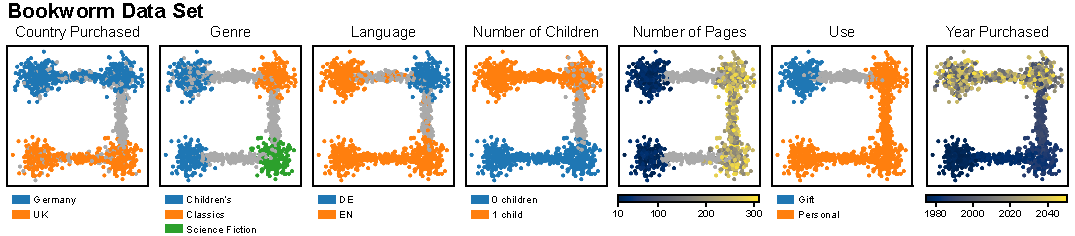
\includegraphics{fig_variable_values.pdf}
  \caption{\label{fig:variable_values}Scatter plots for each feature of our fictional Bookwork dataset. The point positions correspond to the its two-dimensional embedding, revealing four distinct clusters connected by three transitions. Categorical variables are colored with a discrete colormap, while the two numeric variables are colored with a continuous colormap. Missing values are colored gray.}
\end{figure*}

Miller~\cite{Miller2019} posits that the process of explanation involves three cognitive processes: generation, selection, and evaluation. In the context of explaining two-dimensional embeddings, VERA aims to automate the first and second of these three. First, VERA generates several potential explanations -- each of which describes a different pattern in embedding. Second, since some explanations are likely more informative than others, VERA then ranks and selects the most salient explanations. Finally, the selected explanations are shown to the user, with whom the responsibility of evaluating, interpreting, and contextualizing the explanations ultimately rests.

We propose two different types of visual explanations: \textit{constrastive explanations} and \textit{descriptive explanations}.
Constrastive explanations show how the values of a single, high-dimensional feature are distributed across the embedding space.
Descriptive explanations, on the other hand, list the feature values that describe specific regions of the embedding space, e.g., clusters.
Contrastive explanations can help answer questions like ``Where do the different feature values occur?'' while descriptive explanations answer questions like ``What feature values are characteristic for this region?''.

Given an arbitrary data set $D \in \mathbb{R}^{N \times |F|}$ and its corresponding two-dimensional embedding $Y \in \mathbb{R}^{N \times 2}$, our aim is to relate different regions of $Y$ back to the original, high-dimensional features $f \in F$.
Some feature values may be characteristic of specific regions of $Y$, for instance, data points in a particular cluster may all share the same category or contain similar numeric values.
We associate groups of informative values into \textit{rules}, indicating a particular category or numeric interval.
A rule $\varphi_i$ is defined as a function $\varphi: Y \rightarrow \left \{ 0, 1
\right \} $, which evaluates to $1$ if a sample $y$ satisfies the rule condition and $0$ otherwise.
Rules are associated with \textit{regions} via \textit{region annotations} $e_i$, which represent pairs of rules $\varphi_i$ and regions $r_i$, $e_i = \left ( r_i, \varphi_i \right )$.
Each region $R_i$ represents a set of points $R_i = \{ y_1, y_2, \cdots, y_N \} \subseteq Y$ contained within the region.
Region annotations $\{ e_1, e_2, \cdots, e_k \}$ can be merged into \textit{region annotation groups} $e_{\text{group}}$ associated with rule $\varphi_{\text{group}}(y) = \prod_{i=1}^k \varphi_i(y)$ and region $R_{\text{group}} = \bigcup_{i=1}^{k} R_i$. Since region annotation groups serve the same purpose as region annotations, we use the two terms interchangeably.
Once we have identified a set of informative region annotations $E = \left \{ e_1, e_2, \cdots, e_K \right \}$, the next step is to display these to the user. Simultaneously displaying all region annotations to the user in a single image would result in overlapping regions and labels, rendering the visualization unreadable.
Instead, we group region annotations into \textit{panels} $P \subseteq E$ (also referred to as \textit{visual explanations}) and arrange collections of panels into \textit{layouts} $L = \left \{ P_1, P_2, \cdots, P_L \right \}$. A layout is then displayed in a small multiple fashion.

In the upcoming sections, we use a fictional, guiding example to outline the individual steps of our approach.
This fictional dataset, aptly named the Bookworm dataset, comprises of samples corresponding to books owned by an imaginary literary enthusiast. Each book is characterized by seven features: book language, genre, number of pages, year and country of purchase, whether or not the book owners had children at the time of purchase, and whether or not the book was purchased for personal use or as a gift.
Fig.~\ref{fig:variable_values} shows the distribution of feature values as they appear in a specially-designed two-dimensional embedding.

Through these books, we can trace the life of this fictional book collector. The bottom left cluster -- filled with children's books presumably given to them by their parents -- give us a peek into their childhood. Their teenage years are represented by the bottom right cluster, filled with longer science fiction books. After spending their formative years in the United Kingdom, the collector relocates to Germany, where their literary tastes shift to German classics, which remain their favorites to this day. Soon thereafter, they have their first child, in whom they also resolve to instill an appreciation for the literary arts. However, to preserve their child's British heritage, they limit their offspring to a strict diet of English literature.
While this story can be inferred by carefully examining Fig.~\ref{fig:variable_values}, the following sections will show how VERA can produce explanations that uncover this same narrative automatically.

\subsection{Region Construction}
\label{sec:region-construction}

Region annotations are the fundamental building blocks of visual explanations, representing groups of data points in the embedding that share a common characteristic.
In this section, we outline the steps to identify and construct informative region annotations. We discuss how to combine these regions into informative visual explanations in the next two sections.
At a high level, our region construction procedure follows three steps, depicted in Fig.~\ref{fig:region_construction}.

\begin{figure*}[t]
  \centering
  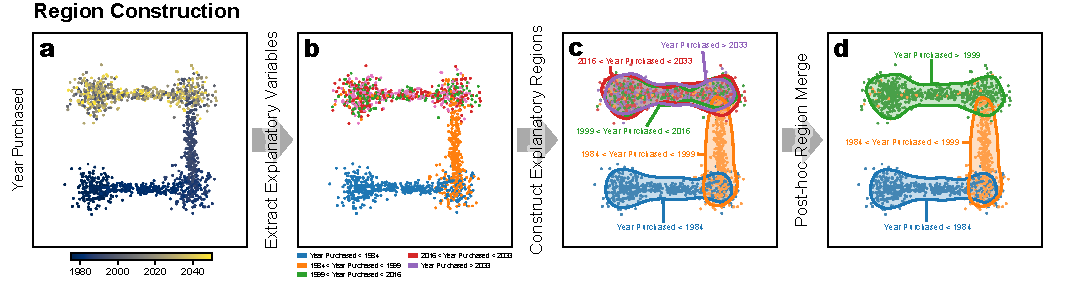
\includegraphics{fig_construct_regions.pdf}
  \caption{\label{fig:region_construction}We illustrate the region construction process for a single feature using a synthetic example. (a) Two-dimensional embeddings are often inspected by coloring points by their corresponding feature values. (b) We discretize the numeric values into five bins, resulting in five binary indicator variables. Here, points here are colored according to their discretization bin membership. (c) For each of the discretized bins, we extract regions by tracing the contours of the corresponding KDE. (d) Finally, we merge ovelapping regions to obtain more informative and readable visualization.}
\end{figure*}

\subsubsection{Extracting Explanatory Variables}
\label{sec:discretization}

An input data set $D$ can include both categorical and numeric features.
For categorical features, we apply one-hot encoding, indicating each sample's membership to a particular category in $k$ binary indicator variables.
For numeric features, we use \mbox{$k$-Means} quantization to discretize their values into $k$ bins, each represented by a binary indicator variable indicating whether a sample falls within that bin.
For example, the numeric feature in Fig.~\ref{fig:region_construction}.a is discretized into five bins, with Fig.~\ref{fig:region_construction}.b indicating bin membership using color.
We apply these transformations to each input feature, associating each resulting indicator variable with a rule $\varphi_i$ that specifies its discretization interval or category assignment.
The procedure results in a collection of binary indicator variables which form the basis for constructing region annotations.

\subsubsection{Constructing Region Annotations}

Having obtained a collection of binary indicator variables and their associated rules, we next determine where their corresponding samples appear in the embedding. 
For each variable, we obtain its kernel density estimate (KDE) $D$ using a Gaussian kernel.
If sample-wise distortion measures of the embedding are provided, we incorporate them as weights during the estimation step to avoid generating explanations of poorly mapped samples in the embedding space\footnote{These regions likely correspond to spurious artifacts of the dimensionality reduction process rather any true underlying structure}.
Next, we extract contour lines of the KDE at a user-specified level and use the resulting polygons as our visual representation of a region $r_i$. By default, we extract contour lines at $0.25 \cdot \max D$.
By construction, each resulting region encompasses samples that predominantly share a particular feature value.
In our running example, the five categories corresponding to discretization bins in Fig.~\ref{fig:region_construction}.b are used to construct the five corresponding regions shown in Fig.~\ref{fig:region_construction}.c.
We then combine the obtained rules and regions into region annotations $e_i = \left( r_i, \varphi_i \right)$, which serve as the building blocks for constructing visual explanations.

An important consideration of the KDE step is setting the Gaussian kernel bandwidth $\sigma$.
Different embedding algorithms produce embeddings that can span across different scales, e.g., one embedding may span from $-1$ to $1$ along its dimensions, while another may span from $-10$ to $10$.
Additionally, a single scale parameter is unlikely to be appropriate for data sets containing different numbers of samples. For instance, in a dataset with 50 samples, we are likely to be interested in groups of 10-20 points, while in a dataset containing 2 million samples, the groups of interest are likely larger.
By default, we set $\sigma$ to equal the median distance of each point's $k$-th nearest neighbor, setting $k=\sqrt{N}$.
Intuitively, the scale parameter controls the granularity of the obtained region anntations:
small values lead to a larger number of smaller regions revealing fine-grained details, while large values generate larger regions, resulting in more high-level explanations.

\subsubsection{Post-hoc Region Merging}
\label{sec:post-hoc-merge}

When constructing explanatory variables, we assign each sample to one of the resulting binary indicator variables, indicating its membership to a particular category or value range.
However, it is common for samples belonging to different groups to occupy the same regions of the embedding space.
For example, the discretization step in Fig.~\ref{fig:region_construction}.c assigns the samples in the top part of the embedding into three separate region annotations.
However, spatially, these regions exhibit near perfect overlap and, upon inspecting their associated rules, we find that they could be consolidated into a single region annotation.
Merging these kinds of regions reduces the number of rules and regions, simplifying the resulting visual explanations and, ultimately, reduces the cognitive load on the end user.

In order to identify and merge overlapping and semantically related regions, we develop a post-hoc merging procedure.
Our procedure identifies overfragmented features and consolidates them into a single region annotation.
For a set of region annotations to be merged, they must satisfy two criteria: high spatial overlap and compatibility between their rules.

Determining the semantic compatibility of rules is straightforward. For rules derived from ordinal or numeric features, only consecutive bins or categories may be merged. For rules originating from nominal categorical features, any combination of categories can be merged.

Determining the degree of spatial overlap between two regions is similarly straigthforward.
We define the \textit{maximum overlap} between two regions $r_i$ and $r_j$ as
\begin{equation}
\text{max\_overlap}(r_i, r_j) = \max \left \{ \frac{|r_i \cap r_j|}{|r_i|}, \frac{|r_j \cap r_i|}{|r_j|} \right \}, \notag
\end{equation}
where $|r|$ denotes the number of samples within that region.
A pair of regions can be merged if their maximum overlap exceeds a predetermined threshold.
This formulation ensures that small regions, which are completely encompassed by a larger region, can be absorbed into the larger region.

Following the merging step, features with little or no spatial correlation will end up with a single region annotation, covering the entire embedding and encomapssing all feature values. This is because, for these features, their values are spread evenly across the embedding space and the region construction step produces overlapping regions that extend across the entire embedding space, which the merging procedure promptly puts back together.
Since these singleton region annotations provide no meaningful information about the structure of the embedding space, we discard them from subsequent analysis.

In our running example, the three region annotations in the top of Fig.~\ref{fig:region_construction}.c exhibit near-perfect overlap and their associated rules are semantically compatible. Therefore, the three regions can be merged into a single region annotation, shown in Fig.~\ref{fig:region_construction}.d.

\subsection{Contrastive Explanations}
\label{sec:contrastive}

Contrastive explanations show how the values of a particular feature are distributed across the embedding space.
While conceptually similar to coloring points based on their feature values, our approach automatically filters out spatially irrelevant features and ranks the remaining ones according to their informativeness in explaining the observed patterns. This allows users to focus on the most relevant features without having to manually sift through potentially large numbers of available features.
%Second, color scales based on numeric values are often skewed by extreme values, making the resulting visualizations difficult to read. Although such distortions are easily corrected, they remain a common nuisance. The discretization step described in Section~\ref{sec:discretization} eliminates this problem entirely, ensuring clearer visualizations without additional user effort.

\subsubsection{Explanation Construction}

Constructing contrastive visual explanations is straightforward: we simply include all region annotations $e_i$ associated with a particular feature $f$.
However, even after filtering, we may still need be left with a large number of candidate explanations.
To further reduce the number of candidate visual explanations, we develop a procedure to automatically identify and merge features with a high degree of spatial overlap.

The \textit{contrastive merge} combines features with near-perfectly spatially overlapping region annotations. Unlike the post-hoc merging procedure described in Section~\ref{sec:post-hoc-merge}, which merges only region annotations derived from a single feature, the contrastive merge combines region annotations derived from multiple different features.
In order to combine two feature explanations $f_1$ and $f_2$, we require that each associated region annotations $e_i \in f_1$ have a nearly perfectly spatially overlapping counterpart $e_j \in f_2$. If such a bipartite matching is found, we merge the matching pairs of region annotations, effectively representing two features using a single collection of region annotations.
For example, the left panel in Fig.~\ref{fig:contrastive_merge} depicts two separate features whose region annotations exhibit near-perfect overlap and can be merged into a single explanation shown on the right.
This procedure not only reduces the number of candidate visual explanations, but describes more features using fewer panels and reveals relationships between high-dimensional features.

\begin{figure}[t]
  \centering
  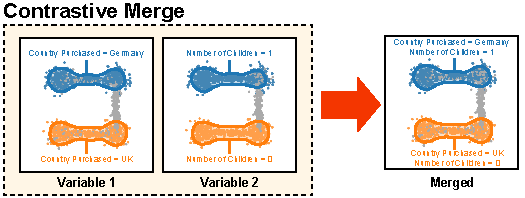
\includegraphics{fig_contrastive_merge.pdf}
  \caption{\label{fig:contrastive_merge}The contrastive merge. If two features contain region annotations that have a nearly perfect overlap bipartite matching, we can merge the two features into one. This not only reduces the number of panels a user needs to inspect but also reveals relationships between features.}
\end{figure}


\subsubsection{Explanation Selection}
\label{sec:contrastive-selection}

To identify contrastive explanations most likely to be informative to end users, we rank and select visual explanations according to three criteria: the total region overlap, mean purity, and the human attention score.

Visual explanations describing features whose values are localized to particular regions of the embedding space are likely to be more informative than features with values spread evenly across the embedding space. Region annotations associated with highly-localized features exhibit lower overlap between their regions than those associated with evenly distributed features.
We compute the overlap between two region annotations as the Jaccard similarity of their regions and define the \textit{total region overlap} of a panel $P$ by taking the mean overlap between all pairs of included region annotations $(e_i, e_j)$.

The purity of each region annotation indicates what proportion of the samples encompassed by the region satisfy its associated rule:
\begin{equation}
\text{purity}(r) = \frac{1}{|r|} \sum_{y_i \in r} \varphi_i (y_i). \notag
\end{equation}
High-purity regions signify a stronger spatial pattern than low-purity regions, and should be preferred. For each panel, we compute the \textit{mean purity} of the contained explanatory variables.

A well-known finding from psychology states that human working memory has limited capacity and can pay attention to only a handful of items at a time. Several bounds have been proposed, including seven~\cite{Miller1956}, four~\cite{Cowan2001}, and two~\cite{Gobet2004}. Panels containing large numbers of region annotations are more likely to overwhelm the user, therefore, panels with fewer region annotations should be preferred. We define the \textit{human attention score} $\left | 3 - |P| \right |$ where $|P|$ denotes the the number of contained region annotations in panel $P$ and assigns lower scores to panels containing three region annotations. In our case, three serves as our intermediate estimate of how many items a user can comfortably reason about at the same time. 

We compute panel rankings for each of these three metrics and compute a weighted sum to obtain a final ranking. We then select the top $k$ panels with the highest overall ranking as our final contrastive explanations. This process is illustrated in Fig.~\ref{fig:contrastive_generation}.

\begin{figure}[t]
  \centering
  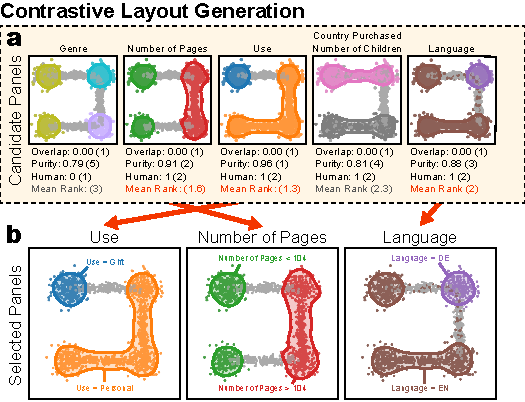
\includegraphics{fig_contrastive_selection.pdf}
  \caption{\label{fig:contrastive_generation}Contrastive layout generation. (a) Generating candidate panels simply involves including all explanatory variables associated with a particular feature in a separate panel. Each candidate panel is scored and ranked according to three metrics, and a weighted mean rank is computed for each panel. (b) The top $k$ panels with the highest mean rank, indicated in red, are included in the resulting layout.}
\end{figure}


\subsection{Descriptive Explanations}

Descriptive explanations describe regions of the embedding space by determining sets of features and their values that are characteristic for specific regions in the embedding space. Unlike contrastive explanations, which primarily focus on explaining single features, descriptive explanations identify combinations of feature values localized in the same regions of the embedding space, potentially characterizing specific groups of samples.

\subsubsection{Explanation Construction}

\begin{figure}[t!]
  \centering
  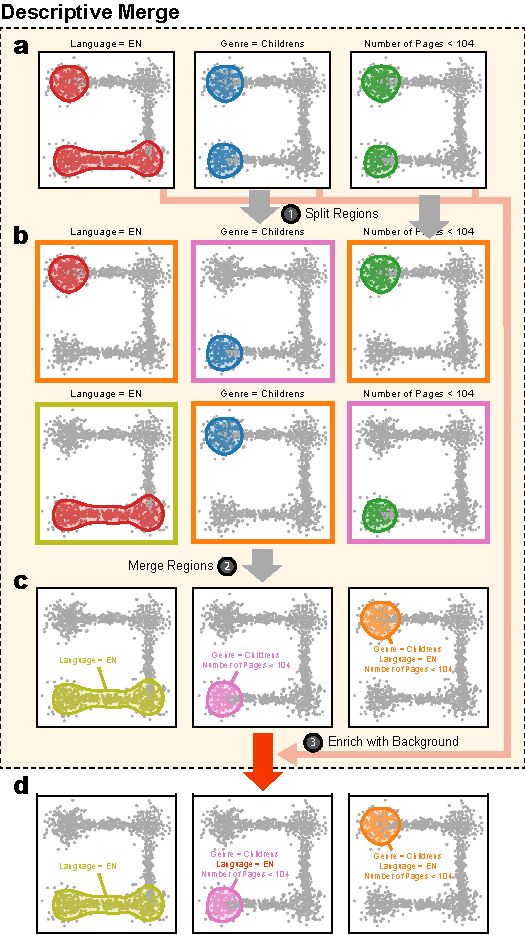
\includegraphics{fig_descriptive_merge.pdf}
  \caption{\label{fig:descriptive_merge}The descriptive merge. In this example, we consider a subset of three explanatory variables (a). In the first step, we split explanatory variable into disjoint regions (b). Then, we identify spatially overlapping explanatory variables and merge them into explanatory variable groups (c). In the final step, each explanatory variable group is imbued with background explanatory variables (d). In this instance, the middle panel depicting the pink region receives an additional, background descriptor, highlighted in red.}
\end{figure}

As in contrastive explanation construction, the regions produced by the procedure outlined in Section~\ref{sec:region-construction} serve as a good starting point for generating explanations, but can be further refined to convey descriptive information using the \textit{descriptive merge}.

The \textit{descriptive merge} comprises of three basic steps. In the first step, we split region annotations comprised of multiple disjoint regions into separate region annotations. For instance, the three region annotations shown in Fig.~\ref{fig:descriptive_merge}.a each contain two disjoint regions, each of which is split into two explanatory variables in Fig.~\ref{fig:descriptive_merge}.b.

After splitting disjoint regions, we next identify and group sets of overlapping region annotations into region annotations groups. 
Two region annotations can be merged if their regions $r_i$ and $r_j$ exhibit a sufficiently high degree of \textit{minimum overlap}:
\begin{equation}
\text{min\_overlap}(r_i, r_j) = \min \left \{ \frac{|r_i \cap r_j|}{|r_i|}, \frac{|r_j \cap r_i|}{|r_j|} \right \}. \notag
\end{equation}

This approach is similar to the post-hoc merging procedure described in Section~\ref{sec:post-hoc-merge}, where we required the maximum overlap to exceed a particular threshold. There, the maximum overlap metric ensured that smaller region annotations could be absorbed into larger, encompassing region annotations. Here, this approach would generate misleading annotations. Consider two region annotations $e_i$ and $e_j$ associated with rules $\varphi_i, \varphi_j$ and regions $r_i, r_j$ respectively. If $r_j$ corresponds to a small region, entirely contained within the larger region $r_i$, the merged rule $\varphi_{\text{new}}$ would indicate that the points within the new region satisfy both rules $\varphi_i$ and $\varphi_j$. Because the new region $R_{\text{new}}$ contains points from both $r_i$ and $r_j$, a large proportion of points in $e_{\text{new}}$ would not satisfy rule $\varphi_j$ and would be misleading. 

The merged regions produced in the previous step contain rules originating from regions with nearly perfect overlap. However, these new regions can be subsets of larger regions with their own associated rules. In the third step, provided the regions achieve a sufficiently high minimum overlap, we add rules from larger regions to the smaller, newly formed ones. Importantly, we do not merge the regions; we only add rules to the smaller regions.
For example, the pink region in the middle panel of Fig.~\ref{fig:descriptive_merge}.c represents shorter children's books, obtained by merging the perfectly overlapping regions in Fig.~\ref{fig:descriptive_merge}.b highlighted in pink. However, these books are also contained within the yellow region in the left panel of Fig.~\ref{fig:descriptive_merge}.c, which corresponds to English books. The pink cluster in Fig.~\ref{fig:descriptive_merge}.c can therefore be enriched with the rule from the yellow cluster. The resulting explanatory variable is shown in Fig.~\ref{fig:descriptive_merge}.d. We refer to this process as \textit{background enrichment}.

\subsubsection{Explanation Selection}

\begin{figure*}[t!]
  \centering
  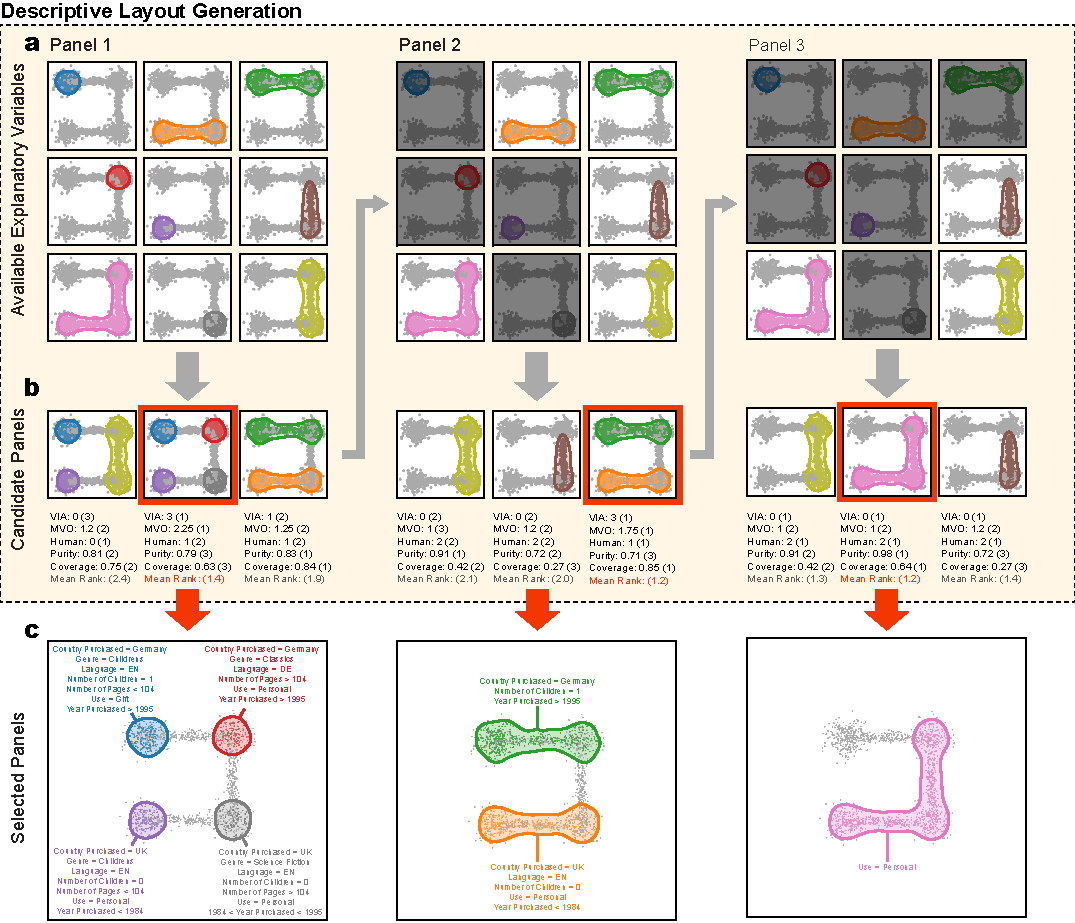
\includegraphics{fig_descriptive_selection.pdf}
  \caption{\label{fig:descriptive_generation}The descriptive layout generation follows an iterative approach. Given a set of available explanatory variables in (a), we identify non-overlapping combinations of these to be used as candidate panels. We show three such candidate panels in (b). Then, each panel is scored along five different metrics, which are subsequently ranked and averaged. The panel with the highest mean rank, indicated in red, is added to the resulting layout, shown in (c). Finally, we remove the explanatory variables in the selected panel from the set of available explanatory variables. We then repeat the procedure until we generate a specified number of panels or until we run out of explanatory variables.}
\end{figure*}

Descriptive explanations are generated and selected in an iterative fashion.
Given an initial set of available explanatory variables $S_0$, we first identify all potential combinations of explanatory variables such that the overlap between regions does not exceed some user-specified threshold. We cast this as an independent set problem, where each node in the graph corresponds to a particular explanatory variable, and edges are placed between them where the overlap between their corresponding regions exceeds the threshold. The independent sets of this graph correspond to collections of spatially non-overlapping regions, which are then considered candidate panels.

A key consideration when generating descriptive explanations is how to enforce the principles of contrastive explanation.
In contrastive explanations, the panels show regions of different values for individual features and are contrastive by nature.
Here, however, each panel can contain explanatory variables comprised describing different features. In this case, a user may not be able to compare regions with one another within a single panel, as the different regions may correspond to different features.

To enforce a level of contrastivity, we score each panel according to its \textit{mean variable occurrence} (MVO). The MVO counts the occurrence of each included feature in the explanatory variables and reports the mean value. A high MVO indicates that the many of the included features appeared in multiple explanatory variables. If a feature appears in all explanatory variables, we assign a special  \textit{variable in all} (VIA) score of 1 and 0 otherwise.

Additionally, we score each panel according to its \textit{sample coverage}, i.e., what proportion of all data points are contained within any given region in the panel. We also include the \textit{mean purity} and \textit{human attention score} from Section~\ref{sec:contrastive-selection}, preferring panels with high-purity regions and panels with a manageable number of explanatory variables.

In order to select the best panel, we apply the same weighted rank-based approach as in Section~\ref{sec:contrastive-selection} to the five metrics described above.
We insert the most highly-ranked panel $P_{\text{max}}$ into the resulting layout, and the explanatory variables $e_i \in P_{\text{max}}$ are removed from the set of available explanatory variables $S_{t + 1} = S_{t} \setminus P_{\text{max}}$. We repeat the procedure until we generate the requested number of panels $k$ or until we run out of available explanatory variables $S$. The procedure is illustrated in Fig.~\ref{fig:descriptive_generation}.


\section{Usage Scenarios}
\label{sec:case-studies}

To demonstrate the versatility and effectiveness of VERA, we present the generated explanations across several diverse datasets.

\subsection{IBM Employee Attrition Dataset}

We begin with a detailed analysis of the IBM Employee Attrition dataset~\cite{IbmEmployeeAttrition} demonstrating how VERA explanations can help understand the visual patterns in a given two-dimensional embedding. The data set describes 1,470 fictional employees characterized by 33 features. We obtain a two-dimensional embedding using the t-SNE algorithm using the \textsf{openTSNE} library~\cite{Policar2024}.

\begin{figure*}[t]
  \centering
  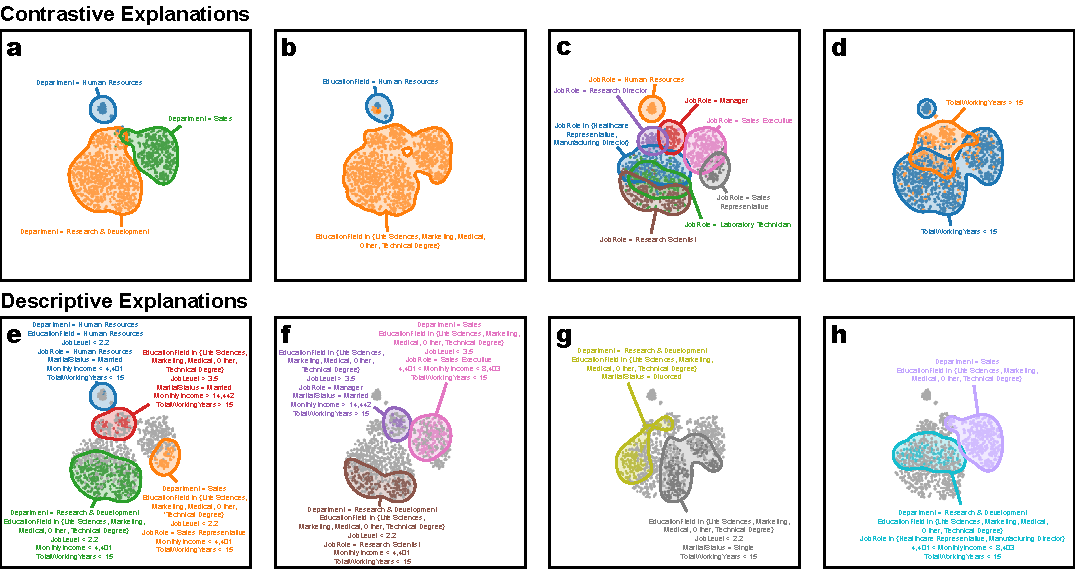
\includegraphics{case_study-attrition.pdf}
  \caption{\label{fig:attrition}Explanations of the IBM Employee Attrition data set. Panels (a-d) show four contrastive explanations corresponding to the features that are spatially most correlated with this particular embedding. The descriptive explanations shown in panels (e-h) characterize different regions of the embedding space.}
\end{figure*}

Fig.~\ref{fig:attrition} shows the top four contrastive and descriptive explanations selected by VERA.
The first two contrastive explanations in Figs.~\ref{fig:attrition}.a and b reveal that the three clusters are primarily distinguished by employees' departments and education fields.
Fig.~\ref{fig:attrition}.c shows that the three clusters can be further subdivided into specific job roles, while Fig.~\ref{fig:attrition}.d shows that the number of total working years also corresponds to the samples' spatial positions.
These four panels alone already help us assign interpretations to the three clusters uncovered by the t-SNE algorithm.

The descriptive explanations depicted in Figs.~\ref{fig:attrition}.e-h offer descriptions of specific regions of the embedding space. For instance, the blue cluster in Fig.~\ref{fig:attrition}.e lists the characteristics of the human resources department and primarily includes junior, married employees with alower salaries. In contrast, the red cluster contains more senior, married individuals with higher salaries. Cross-referencing this Fig.~\ref{fig:attrition}.c, we can see that the majority of the employees in the red cluster hold managerial or research director roles. We can similarly inspect the other regions to gain further insight into the structure captured by the embedding.

Notice that many of the identified regions in Fig.~\ref{fig:attrition} do not correspond to discrete clusters but rather represent regions within or across clusters. For instance, the gray region in Fig.~\ref{fig:attrition}.g corresponds to single employees with less than 15 years of experience and low job levels -- likely younger, junior staff. On the other hand, them yellow region primarily includes divorced employees. We are provided with no information about their job level or total working years. Therefore, we do not assume any particular values about these employees. This allows VERA to highlight and explain interesting parts of clusters.

\subsection{Abalone Dataset}

\begin{figure}[htb]
  \centering
    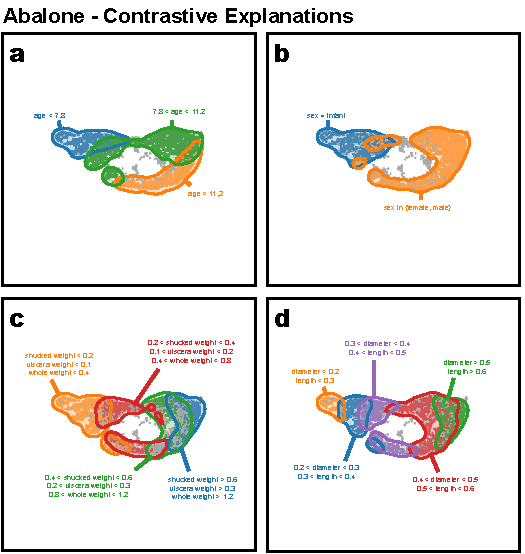
\includegraphics{case_study-abalone.pdf}
    \caption{\label{fig:abalone}Contrastive explanations for a UMAP embedding of the Abalone dataset. Panels (a-d) highlight selected features, showing the spatial distribution of age, sex, and physical measurements, as well as correlations between features related to animal weight and size.}
\end{figure}

The Abalone dataset~\cite{Nash1994} is a well-known benchmark in regression tasks, containing 4,177 samples of abalones -- marine mollusks with distinctive ear-shaped shells. Each sample is characterized by eight features, including physical measurements of the body and shell, as well as biological attributes such as age and sex. We generate a two-dimensional embedding with the UMAP algorithm using the \textsf{umap-learn} library~\cite{McInnes2018}. The obtained embedding reveals no distinct clusters, but forms an elongated shape stretching from left to right.

Fig.~\ref{fig:abalone} shows selected contrastive explanations generated by VERA.
The explanations reveal that the elongated shape reflects the size and age of the abalones: younger abalones are smaller and lighter, while older abalones are larger and heavier. Fig.~\ref{fig:abalone}.b also suggests that the sex of the animals does not affect its size.
Figs.~\ref{fig:abalone}.c and d highlight the benefits of the contrastive merge procedure. Fig.~\ref{fig:abalone}.c combines shucked weight, viscera weight, and whole weight into a single explanation, while Fig.~\ref{fig:abalone}.d combines shell diameter and length.
This example illustrates how VERA can reduce the number of feature explanations analysts need to examine -- in this case from five to two -- while simultaneously revealing strong correlations between different sets of variables.

\subsection{Iris and Penguin Datasets}

\begin{figure}[ht]
  \centering
  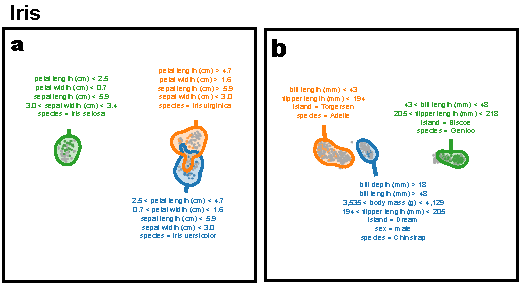
\includegraphics{case_study-iris-penguins.pdf}
  \caption{\label{fig:iris-penguins}Descriptive explanations of the Iris (a) and Penguin (b) data sets. Each explanation provides a comprehensive, high-level overview of the clusters revealed in the embedding.}
\end{figure}

The Iris~\cite{Anderson1936} and Penguin~\cite{Horst2020} datasets are widely used benchmarks in data visualization and machine learning due to their clear clustering strcuture and overall simplicity.
Fig.\ref{fig:iris-penguins} shows one descriptive explanation for each data set, each of which provides a complete overview of the main patterns and relationships.
In the Iris dataset (Fig.~\ref{fig:iris-penguins}.a), VERA identifies regions corresponding to the three species of iris flowers, each characterized by distinct combinations of sepal and petal measurements. For the Penguin dataset (Fig.~\ref{fig:iris-penguins}.b), VERA identifies clusters representing the three penguin species, separated by features such as flipper length and body mass.
For simple data sets such as these comprising relatively few features and having relatively well-defined clusters, a single descriptive explanation can be sufficient to capture the fully convey the structure of the embedding.


\section{User Evaluation}
\label{sec:user-study}

To evaluate the effectiveness of our approach, we conducted a comparative user study comparing the speed and accuracy with which users could reason about low-dimensional embeddings using both an interactive data exploration tool and our newly proposed static VERA explanations.

\subsection{Study Design}

We select the Orange data mining toolkit~\cite{Demsar2013} as our interactive tool of choice because of its ease of use and focus on visual data exploration.
While not explicitly designed for interpreting embeddings, Orange includes standard visualization tools for exploring two-dimensional embeddings. Many related approaches based on feature distribution plots~\cite{Stahnke2016,Eckelt2022} and disciminative models~\cite{Bibal2021,Marcilio2021} can be easily reproduced in Orange using only a handful of widgets.
%A typical workflow for interpreting a specific cluster might involve loading data, embedding and visualizing it in scatter plot, selecting groups of points, and comparing their feature distributions to the remaining samples using a box plot.

We prepare two sets of three real-world data sets each, with varying complexity.
The first data set group $D_1$ comprises the Iris~\cite{Anderson1936}, Employee Attrition~\cite{IbmEmployeeAttrition}, and Raisin~\cite{RaisinDataset} data sets. The second data set group $D_2$ includes the Penguins~\cite{Horst2020}, Titanic~\cite{Dawson1995}, and Wine Quality~\cite{Cortez2009} data sets. For each data set, participants were asked to answer a series of typical questions during the exploration of two-dimensional embeddings, e.g., ``What makes this cluster different from the remaining clusters?'', ``What characterizes the samples in this cluster?'', and ``Do you notice any trend along this region?''.

We recruited 57 bachelor's students enrolled in the Introduction to Machine Learning course at the Faculty of Computer and Information Science at the University of Ljubljana.
Prior to the study, the participants had some familiarity with Orange but were not familiar with VERA explanations. Before conducting the study, we provided a short tutorial on both Orange and VERA explanations.
We randomly assigned participants to one of two user groups. The first group $G_1$ first used Orange to answer questions related data sets $D_1$, then used VERA explanations for questions relating to data sets in $D_2$. Conversely, the second group $G_2$ first used VERA to answer questions relating to $D_1$, then used Orange to answer questions relating to the data sets in $D_2$. On average, students answered $29.2$ of the $32$ questions ($\text{SD}= 4.3$, $\text{SE}=0.56$), amounting to a total of $1,666$ responses.

To asses the participant's response time and accuracy, we timed how long it took each participant to answer each question related to a particular data set group and determined whether they answered the questions correctly. Upon completing both data set groups, we asked participants to answer a final questionnaire in which they could provide feedback related to the two tools.

\subsection{Results}

The results of our study show that participants using VERA explanations performed as well as participants using Orange, but taking significantly less time.
The difference in user performance was not statistically significant (t-test $p=0.084$), with 91\% ($\text{SE}=0.9\%$) of participants answering correctly when using Orange and 93\% ($\text{SE}=1.0\%$) when using VERA.
On the other hand, participants in both user groups answered questions significantly faster when using VERA explanations ($p<0.005$). On average, participants using Orange took $29$ minutes ($\text{SD}= 11.5$, $\text{SE}=2.1$) to complete questions related to $D_1$ and $23$ minutes ($\text{SD}= 6.0$, $\text{SE}=1.1$) to complete questions related to $D_2$. Conversely, participants using VERA explanations required $21$ minutes ($\text{SD}= 6.3$, $\text{SE}=1.2$) and $15$ minutes ($\text{SD}=5.4$, $\text{SE}=1.1$) for each data set group, representing an increase in speed of approximately 33\%.
These results confirm that participants in both groups were able to answer the questions with roughly the same degree of accuracy, but at a much faster rate when using VERA explanations.

Interestingly, when asked about the number of characteristic or distinguishing features, participants often mentioned more features when using VERA explanations ($p=0.04$). When generating explanations using Orange, participants mentioned an average of $2.0$ ($\text{SD}= 1.29$, $\text{SE}=0.07$) features in their answers, while this increased to $2.2$ ($\text{SD}= 1.33$, $\text{SE}=0.07$) when using VERA explanations. This discrepancy could be due to several factors. For example, when exploring two-dimensional embeddings with an interactive tool, users typically have to manually sift through the many different features to explore their correspondence to the embedding space. Participants often stop their exploration after identifying one or two informative features, potentially missing other equally informative features. VERA explanations, on the other hand, provide all relevant explanations at once. While these explanations are limited in the number of features they display, the explanation ranking mechanisms in VERA ensure that the user sees the most salient features first. Thus, the user simply \textit{sees} all the features and cannot miss them by accident.

In the final feedback questionnaire, we asked participants to document their experience with both tools. Consistent with our quantitative results, most participants (91\%, $\text{SE}=4\%$) reported that they were able to answer questions more quickly using the VERA explanations. The majority of participants (77\%, $\text{SE}=6\%$) also confirmed that the static explanations provided were just as informative as Orange.
Surprisingly, when asked which tools they trusted more, 50\% ($\text{SE}=8\%$) of participants said they trusted both tools equally, 20\% ($\text{SE}=6\%$) said they trusted VERA explanations more, and 30\% said they trusted Orange more ($\text{SE}=7\%$). 
We expected that users would tend to trust full-featured, interactive toolkits like Orange more than static visual explanations because these tools provide users with multiple methods to verify their findings and allow them to drill down into specific parts of the visualization. VERA explanations, on the other hand, are static and offer no such options, forcing the user to simply trust the image.

Finally, we asked participants which types of VERA explanations they found more informative, and asked them to rate each type of explanation for its usefulness on a typical five-point Likert scale. Consistent with Miller's~\cite{Miller2019} findings, most participants (75\%, $\text{SE}=6.6\%$) selected contrastive explanations as the most informative, while 15\% ($\text{SE}=5.4\%$) found both types of explanations equally informative, and 10\% ($\text{SE}=4.7\%$) found descriptive explanations more informative.
Contrastive explanations received a higher overall rating of $4.3$ ($\text{SD}= 0.89$, $\text{SE}=0.13$), while descriptive explanations received a lower overall rating of $3.2$ ($\text{SD}= 1.06$, $\text{SE}=0.16$).
We note that this result does not imply that descriptive explanations are not useful, but merely that users generally find contrastive explanations more informative than descriptive explanations.


\section{Limitations and Future Work}

While we have shown that the visual explanations generated by VERA are useful, there are still a number of limitations to the proposed approach that provide avenues for future research.

The present study considers only tabular data, where each feature conveys some human-readable, semantic meaning. Today, analysts routinely deal with data sets of different modalities, for which our approach may also prove useful.
For example, in compositional data sets such as text corpora and gene expression data, descriptive explanations could be used to identify characteristic groups of words or highly expressed genes for different regions of the embedding space.
Applying our proposed approach to other data modalities, such as image, sound, video, and graph data, where semantically meaningful features are scarce, is not straightforward. For these data modalities, more specialized approaches are likely to be needed to address the needs of each particular modality.

Another limitation of our approach is the issue of scaling as the number of features increases.
The case study highlighted above and the datasets used in the user study contain a maximum of 33 features. As currently designed, VERA would likely struggle to produce meaningful visualizations when faced with hundreds or thousands of features.
For example, contrastive explanations typically show the top $k$ most informative features. As the number of features increases, more panels are needed to get a complete view of all spatially localized features.
Descriptive explanations, on the other hand, suffer from a different limitation. Each descriptive panel typically contains several explanatory variables along with their associated rule descriptors. As we increase the number of total features, the number of rule descriptors also increases, leading to information-dense and eventually incomprehensible labels.
However, with recent advances in natural language processing~\cite{Brown2020,Touvron2023}, we could use large language models (LLMs) to summarize potentially long lists of feature descriptors and display short, automatically generated summaries instead of long feature descriptors. For text data, LLMs could also be used to generate topic descriptions. Where available, ontologies could be used to perform ontology enrichment analysis to identify more semantically meaningful labels. For example, in gene expression data, we could replace long lists of genes with enriched Gene Ontology terms~\cite{GeneOntology2004}, or in drug prescription data, we could replace lists of drugs with enriched Anatomical Therapeutic Chemical codes~\cite{Policar2023}. These can also be summarized by an LLM into a shorter, more human-readable label.
Recent advances in LLM research open up exciting new avenues of research for automatic explanation generation that will benefit not only visual explanations, but the entire field of explicable artificial intelligence as a whole.

A final consideration is that of interactivity. While the development of VERA was motivated primarily by the need for fully automated tools to generate static, visual explanations of two-dimensional embeddings, one can easily envision an interactive system in which visual explanations are integrated into a rich, interactive platform.
Interactive systems allow the user to explore the embedding in much more detail, to focus on subsets of the embedding space, and to drill down into the specific visual structures.
Similar to splatterplots~\cite{MayorgaGleicher2013}, such an interactive system can also take into account the available screen space and dynamically adjust the level of detail shown accordingly.
Such a user interface could be seamlessly integrated into existing visual analytics tools such as Orange~\cite{Demsar2013}, complementing their existing interactive data exploration tools.


\section{Conclusion}

In today's era of large, high-dimensional data sets, unsupervised dimensionality reduction approaches have become essential to exploratory data analysis. These methods help analysts make sense of vast amounts of data, allowing them to visually discover interesting structures in two-dimensional maps and drive hypothesis generation. Recent algorithmic developments have enabled these methods to scale to massive data sets, and it has become commonplace to generate multiple such embeddings using different algorithms and parameter settings, each potentially revealing different facets of the underlying data manifold. However, examining each of these embeddings is time consuming and tedious. Typically, analysts interrogate each embedding in an interactive tool, identifying points of interest, examining their underlying feature distributions, and assigning semantic labels to groups of points.

We present \textit{Visual Explanations via Region Annotation (VERA)}, a fully automated approach for generating static visual explanations of arbitrary two-dimensional embeddings. VERA aims to relate different regions of the embedding space to the original high-dimensional features. Unlike most existing approaches, VERA does not rely on the identification of clusters in the embedding space, but automatically determines potentially interesting regions in the embedding space. Importantly, VERA requires no manual human intervention and can be easily integrated into existing dimensionality reduction pipelines, producing visual explanations as a by-product of the analysis.
VERA produces two complementary types of explanations.
Contrastive explanations identify the most spatially salient features and show where particular feature values occur in the embedding.
On the other hand, descriptive explanations aim at describing certain regions of space in terms of certain high-dimensional feature values.
Drawing on insights from the social sciences, we pay particular attention to ensuring that our explanations follow the principles of contrastivity, so that the resulting explanations are as informative and satisfying as possible.
We validate the utility of our approach through a comparative user study, which shows that our visual explanations are as informative as full-fledged, interactive tools for answering common embedding interpretation tasks. Importantly, however, due to the static nature of our explanations, users are able to gain insight into their embeddings in significantly less time.

Overall, our work contributes to the growing field of interpretable machine learning and offers a new perspective on explaining nonlinear embeddings in terms of their original features.


\section*{Code Availability}

Our open-source, Python implentation of VERA is freely-available at \url{https://github.com/pavlin-policar/vera} and is licensed under the BSD-3 license.


\section*{Acknowledgments}
This work was supported by the Slovenian Research Agency grants P2-0209 and V2-2272.
 
%\bibliography{IEEEabrv,../bib/paper}
\bibliographystyle{ieeetr}
\bibliography{main}

% \newpage

% \section{Biography Section}
% If you have an EPS/PDF photo (graphicx package needed), extra braces are
%  needed around the contents of the optional argument to biography to prevent
%  the LaTeX parser from getting confused when it sees the complicated
%  $\backslash${\tt{includegraphics}} command within an optional argument. (You can create
%  your own custom macro containing the $\backslash${\tt{includegraphics}} command to make things
%  simpler here.)
 
% \vspace{11pt}

% %\bf{If you include a photo:}\vspace{-33pt}
% %\begin{IEEEbiography}[{\includegraphics[width=1in,height=1.25in,clip,keepaspectratio]{fig1}}]{Michael Shell}
% %Use $\backslash${\tt{begin\{IEEEbiography\}}} and then for the 1st argument use $\backslash${\tt{includegraphics}} to declare and link the author photo.
% %Use the author name as the 3rd argument followed by the biography text.
% %\end{IEEEbiography}

% \vspace{11pt}

% \bf{If you will not include a photo:}\vspace{-33pt}
% \begin{IEEEbiographynophoto}{John Doe}
% Use $\backslash${\tt{begin\{IEEEbiographynophoto\}}} and the author name as the argument followed by the biography text.
% \end{IEEEbiographynophoto}

% \vfill

\end{document}
